\chapter{Change of Variables}

\section{Partitions of Unity}

\noindent \textbf{Motivation}:
\begin{itemize}
    \item In order to prove the change of variables theorem, we need a new equivalent definition of the extended integral.
    This definition of integral break the function $f$ up into functions $\phi_Nf$ where $\phi_N$ can be thought of some kind of proportion function, 
    each of which vanishes outside a compact set $S_N$ and we take the limit of the corresponding integrals $\int_Af_N$. It is hard to compute but has many advantages for theoretical purposes such as proving the change of variable theorem.
\end{itemize}

\begin{lemma}
    Let $Q$ be a rectangle in $\R^n$. There is a $C^{\infty}$ function $\phi:\R^n\longrightarrow\R$ such that 
    \begin{equation*}
        \begin{cases}
            \phi(x)>0\text{\quad}x\in Int(Q)\\
            \phi(x)=0\text{\quad otherwise}
        \end{cases}
    \end{equation*}
\end{lemma}

\begin{lemma}
    Let $\mathcal{A}$ be a collection of open sets in $\R^n$. Let $A$ be their union. Then there exists a countable collection $\{Q_1,Q_2,\cdots\}$ of rectangles contained in $A$ such that
    \begin{enumerate}
        \item The sets $Int(Q_i)$ cover $A$.
        \item Each $Q_i$ is contained in an element of $\mathcal{A}$.
        \item (Local finiteness) Each point of $A$ has a neighborhood that intersects only finitely many of the sets $Q_i$.
    \end{enumerate}
\end{lemma}

\begin{definition}
    If $\phi:\R^n\longrightarrow\R$, then the \underline{support} of $\phi$ is defined be the closure of the set $\{x:\phi(x)\neq0\}$.
\end{definition}

\begin{definition}
    Let $\mathcal{A}$ be a collection of open sets in $\R^n$. Let $A$ be their union. A collection of functions $\{\phi_i\}$ is said to be a \underline{partition of unity} on $A$ if it satisfies
    \begin{enumerate}
        \item $\forall x \in A.\phi_i(x)\geq 0$
        \item $S_i=supp(\phi_i)\subset A$
        \item $\forall a\in A.\exists\text{ open $U$ containing $a$ such that $U$ intersects only finitely of $S_i$}$.
        \item $\forall a \in A,\sum_{i=1}^{\infty}\phi_i(a)=1$
    \end{enumerate}
\end{definition}

\begin{theorem}[Existence of partition of unity]\label{existence of partition of unity}
    Let $\mathcal{A}$ be a collection of open sets in $\R^n$. Let $A$ be their union. 
    There exists a sequence $\{\phi_i\}$ of continuous functions $\phi_i:\R^n\longrightarrow\R$ such that
    \begin{enumerate}
        \item $\{\phi_i\}$ is a partition of unity.
        \item $\phi_i$ are of class $C^{\infty}$.
        \item $\{\phi_i\}$ has compact supports.
        \item $\forall i\in\N.S_i\text{ is contained in an element of }\mathcal{A}$.
    \end{enumerate}
\end{theorem}

\noindent\textbf{Example}:
\begin{itemize}
    \item Let $\phi_1:\R\longrightarrow\R$ be defined be the equation
    \begin{equation}
        \phi_1(x)=
        \begin{cases}
            \frac{1+\cos(x)}{2}\text{\quad}-\pi\leq x\leq \pi\\
            0\text{\quad otherwise}
        \end{cases}
    \end{equation}
    For each $m\in\N$, we set
    $$\phi_{2m+1}(x)=\phi_1(x-m\pi)$$
    $$\phi_{2m}(x)=\phi_1(x+m\pi)$$
    Can check that $\{\phi_i\}$ is a partition of unity of $\R$.
    \begin{figure}[ht]
        \centering
        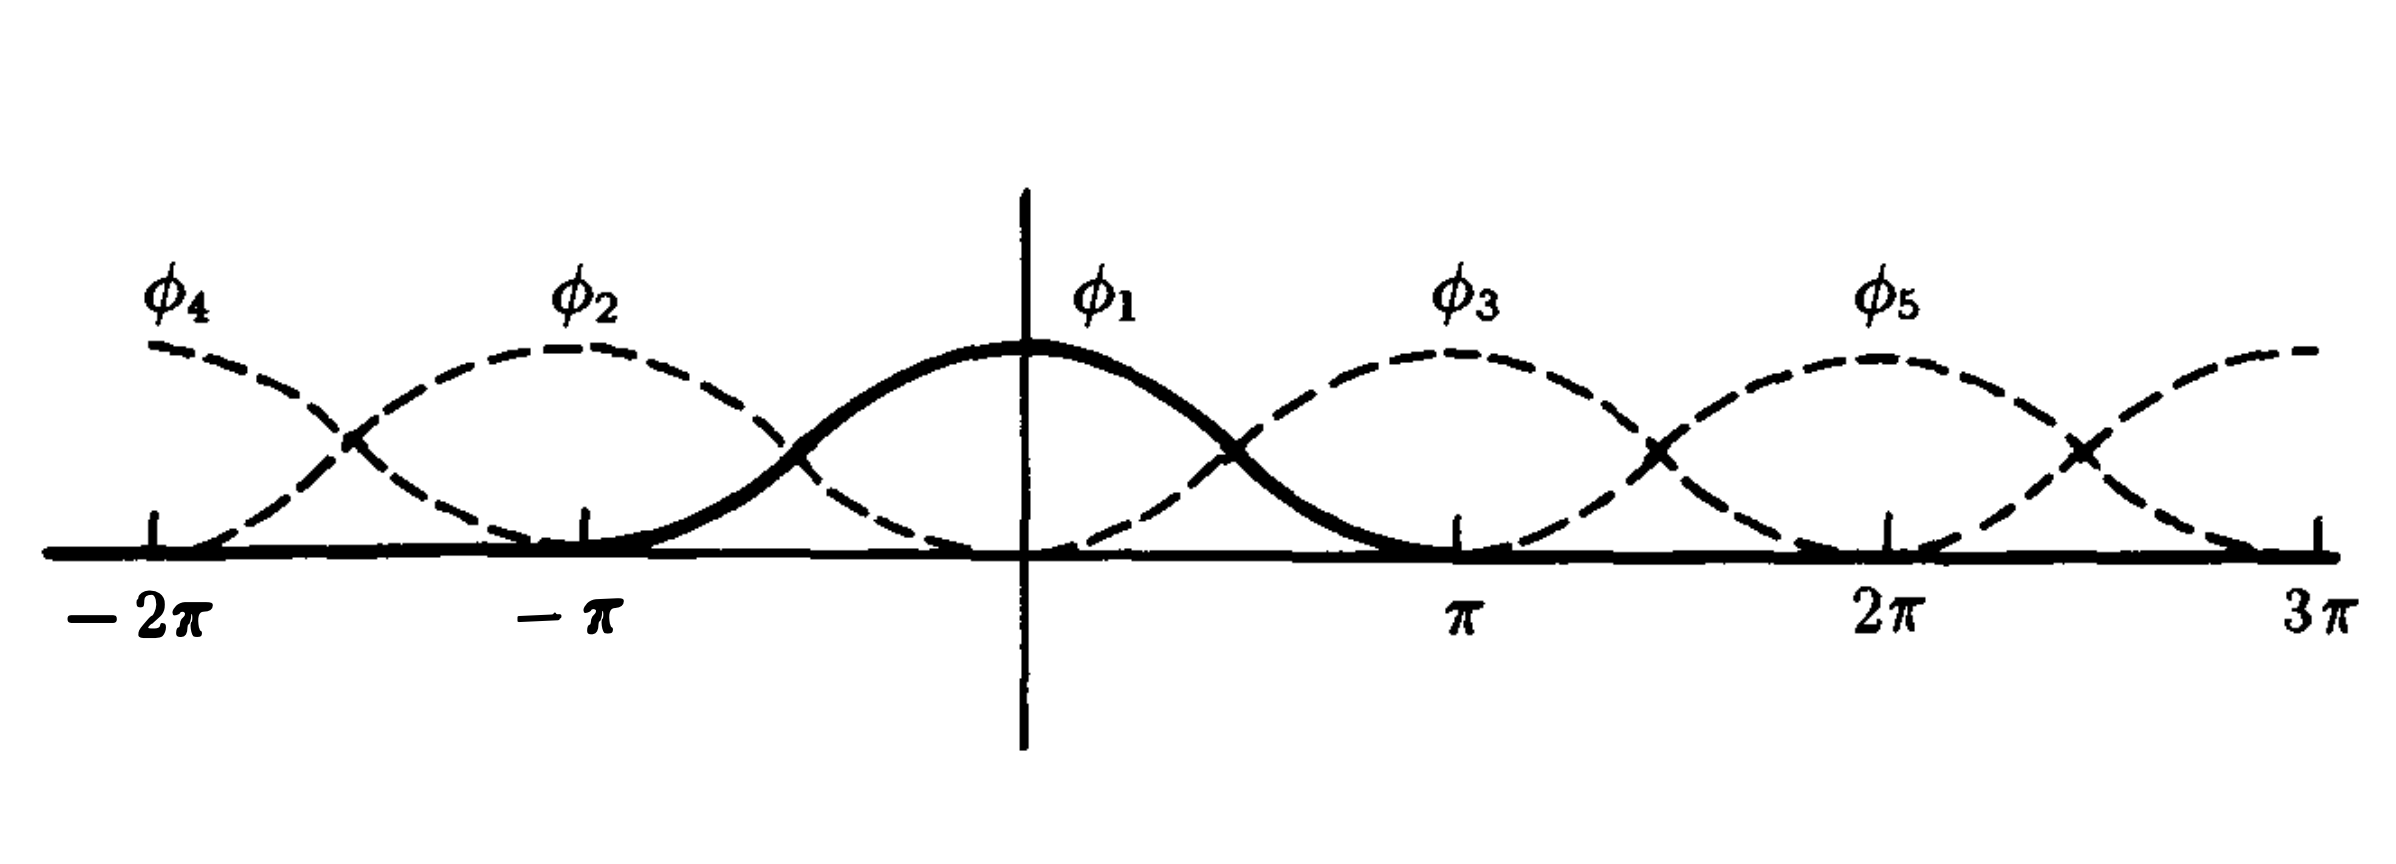
\includegraphics[scale=0.3]{images/Screenshot 2023-01-13 at 21.16.45.png}
        \caption{picture of $\{\phi_i\}$}
    \end{figure}
\end{itemize}

\begin{lemma}
    Let $A$ be opne in $\R^n$. Let $f:A\longrightarrow\R$ be continuous.
    If $f$ vanishes outside the compact subset $C$ of $A$, then the integral $\int_Af$ and $\int_Cf$ exist and are equal.
\end{lemma}

\begin{theorem}[Equivalent definition of extended intrgral 3]\label{Equivalent definition of extended intrgral 3}
    Let $A$ be opne in $\R^n$. Let $f:A\longrightarrow\R$ be continuous. Let $\{\phi_i\}$ be a partition of unity on $A$ having compact supports. The integral $\int_Af$ exists if and only if the series $\sum_{i=1}^{\infty}\int_A\phi_i|f|$ converges. Now
    $$\int_Af=\sum_{i=1}^{\infty}\int_A\phi_if$$
\end{theorem}

\section{Diffeomorphisms in $\R^n$}

\noindent\textbf{Motivation}:
In order to prove the change of variables theorem, we need to obtain two fundamental properties of diffeomorphisms. This we do in the present section.
\begin{itemize}
    \item The image of a compact rectifiable set under a diffeomorphism is another compact rectifiable set.
    \item Any diffeomorphism can be broken up locally into a composite of diffeomorphisms of a special type, called primitive diffeomorphisms.
\end{itemize}

\begin{definition}
    Let $A,B$ be open sets in $\R^n$. Let $g:A\longrightarrow B$ be bijective such that $g$ and $g^{-1}$ are of class $C^r$, then $g$ is called a \underline{diffeomorphism( of class $C^r$)}.
\end{definition}

\begin{lemma}
    Let $A$ be open in $\R^n$. Let $g:A\longrightarrow \R^n$ be a function of class $C^1$. 
    If the subset $E$ of $A$ has measure zero in $\R^n$, then the set $g(E)$ also has measure zero in $\R^n$.
\end{lemma}

\noindent\textbf{Remark}:
\begin{itemize}
    \item Differentiability is needed for the lemma above. If $g$ is merely conntinuous, then the image of a set of measure zero may not have measure zero. Consider the \underline{Peano space-filling curve} $f:[0,1]\longrightarrow[0,1]^2$.
\end{itemize}

\begin{theorem}
    Let $g:A\longrightarrow B$ be a diffeomorphism of class $C^r$, where $A,B$ are open in $\R^n$. Let $D$ be a compact subset of $A$.
    \begin{enumerate}
        \item $g(Int(D))=Int(g(D))\text{ and }g(Bd(D))=Bd(g(D))$
        \item If $D$ is rectifiable, then $g(D)$ is also rectifiable.
    \end{enumerate}
\end{theorem}

\begin{definition}
    Let $h:A\subset \R^n\longrightarrow B\subset \R^n$. Consider the component functions $$h(x)=(h_1(x),\cdots,h_n(x))$$
    We say $h$ is a \underline{primitive diffeomorphism} if $h$ preserves the i-th coordinate for some i.($h_i(x)=x_i$)
\end{definition}

\begin{theorem}
    Let $g:A\longrightarrow B$ be a diffeomorphism of open sets in $\R^n$. Given $a\in A$, there is a neighborhood $U_0$ of $a$ contained in $A$, and a sequence of diffeomorphisms of open sets in $\R^n$
    \begin{equation*}
        \xymatrix{U_0 \ar[r]^{h_1} &U_1 \ar[r]^{h_2} &U_2 \ar[r]^{h_3} & \cdots \ar[r]^{h_k}&U_k} 
    \end{equation*}
    such that the composite $h_k\circ\cdots\circ h_2\circ h_1=g|_{U_0}$ and each $h_i$ is a primitive diffeomorphism.
\end{theorem}

\begin{lemma}
    Let $g:A\longrightarrow B$ be a diffeomorphism of open sets in $\R^n$. Then for every continuous function $f:B\longrightarrow \R$ that is integrable over $B$,
    the function $(f\circ g)|\det(Dg)|$ is integrable over $A$ and
    \begin{equation*}
        \int_Bf=\int_A(f\circ g)|\det(Dg)|
    \end{equation*}
\end{lemma}

\begin{lemma}
    Let $g:A\longrightarrow B$ be a diffeomorphism of open sets in $\R^n$. Let $f:B\longrightarrow \R$ be continuous. 
    If $(f \circ g)|\det(Dg)|$ is integrable over $A$, then $f$ is integrable over $B$.
\end{lemma}

\section{The Change of Variable Theorem}

\begin{theorem}[Substitution rule]
    Let $I=[a,b]$. Let $g:I\longrightarrow\R$ be a function of class $C^1$ with $g'(x)\neq0$ for $x\in(a,b)$.
    Then the set $g(I)$ is a closed interval $J$ with end points $g(a)$ and $g(b)$.
    If $f:J\longrightarrow\R$ is continuous, then $$\int_{g(a)}^{g(b)}f=\int_a^b(f\circ g)g'$$
\end{theorem}

\begin{definition}
    Let $A$ be open in $\R^n$. Let $g:A\longrightarrow\R^n$ be a injective function of class $C^r$, such that $$\forall x\in A.\det(Dg(x))\neq0$$
    Then $g$ is called a \underline{change of variables} in $\R^n$.
\end{definition}

\begin{theorem}
    $g$ is a change of variables in $\R^n$ if and only if $g$ is a diffeomorphism in $\R^n$.
\end{theorem}

\begin{theorem}[Change of variables theorem]\label{Change of variables theorem}
    Let $g:A\longrightarrow B$ be a diffeomorphism of open sets in $\R^n$. Let $f:B\longrightarrow \R$ be a continuous function. 
    Then $f$ is integrable over $B$ if and only if $(f\circ g)\cdot |\det(Dg)|$ is integrable over $A$. In this case 
    $$\int_Bf=\int_A(f\circ g)\cdot |\det(Dg)|$$
\end{theorem}

\section{Applications}

\subsection{Polar, Spherical and Cylindrical Coordinate}

\begin{definition}
    The \underline{polar coordinate transformation} is a function $g:\R^2\longrightarrow\R^2$ defined by 
    $$g(r,\theta)=(r\cos\theta,r\sin\theta)$$
    By computation we have
    \begin{equation*}
        \det(Dg)=\det(\begin{bmatrix}
            D_1g_1 & D_2g_1\\
            D_1g_2 & D_2g_2
        \end{bmatrix})=\det(\begin{bmatrix}
            \cos\theta & -r\sin\theta\\
            \sin\theta & r\sin\theta
        \end{bmatrix})=r(\cos^2\theta+\sin^2\theta)=r
    \end{equation*}
    \begin{figure}[H]
        \centering
        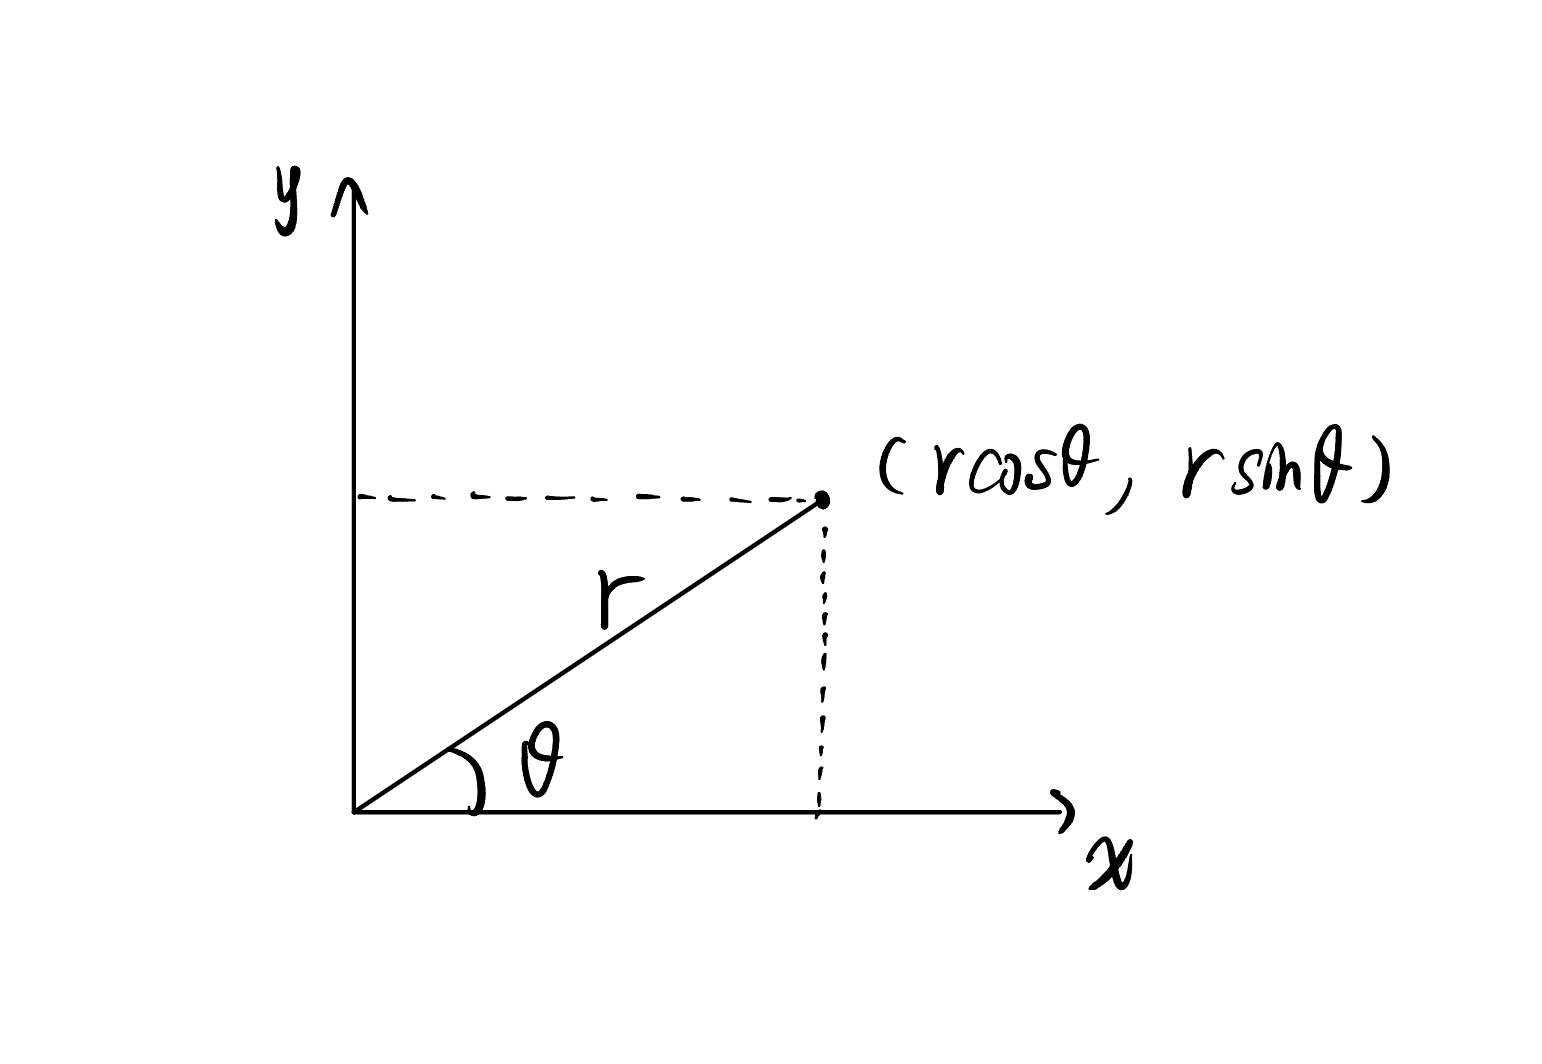
\includegraphics[scale=0.15]{images/IMG_0361.jpg}
        \caption{picture of polar coordinate}
    \end{figure}
\end{definition}
\noindent\textbf{Example}:
\begin{itemize}
    \item Let $B$ be the open set in $\R^2$ defined by $$B=\{(x,y):x>0\text{ and }y>0\text{ and }x^2+y^2<a^2\}$$
    One commonly computes an integral over $B$.i.e. $\int_Bf$ by using the polar coordinate transformation.
    Define the sets $A$ as 
    $$A=\{(r,\theta):0<r<a\text{ and }0<\theta<\frac{\pi}{2}\}$$
    The map $g:A\longrightarrow B$ is a diffeomorphism. The change of variables theorem implies that $$\int_Bf=\int_Af(r\cos\theta,r\sin\theta)\cdot r$$
    \begin{figure}[H]
        \centering
        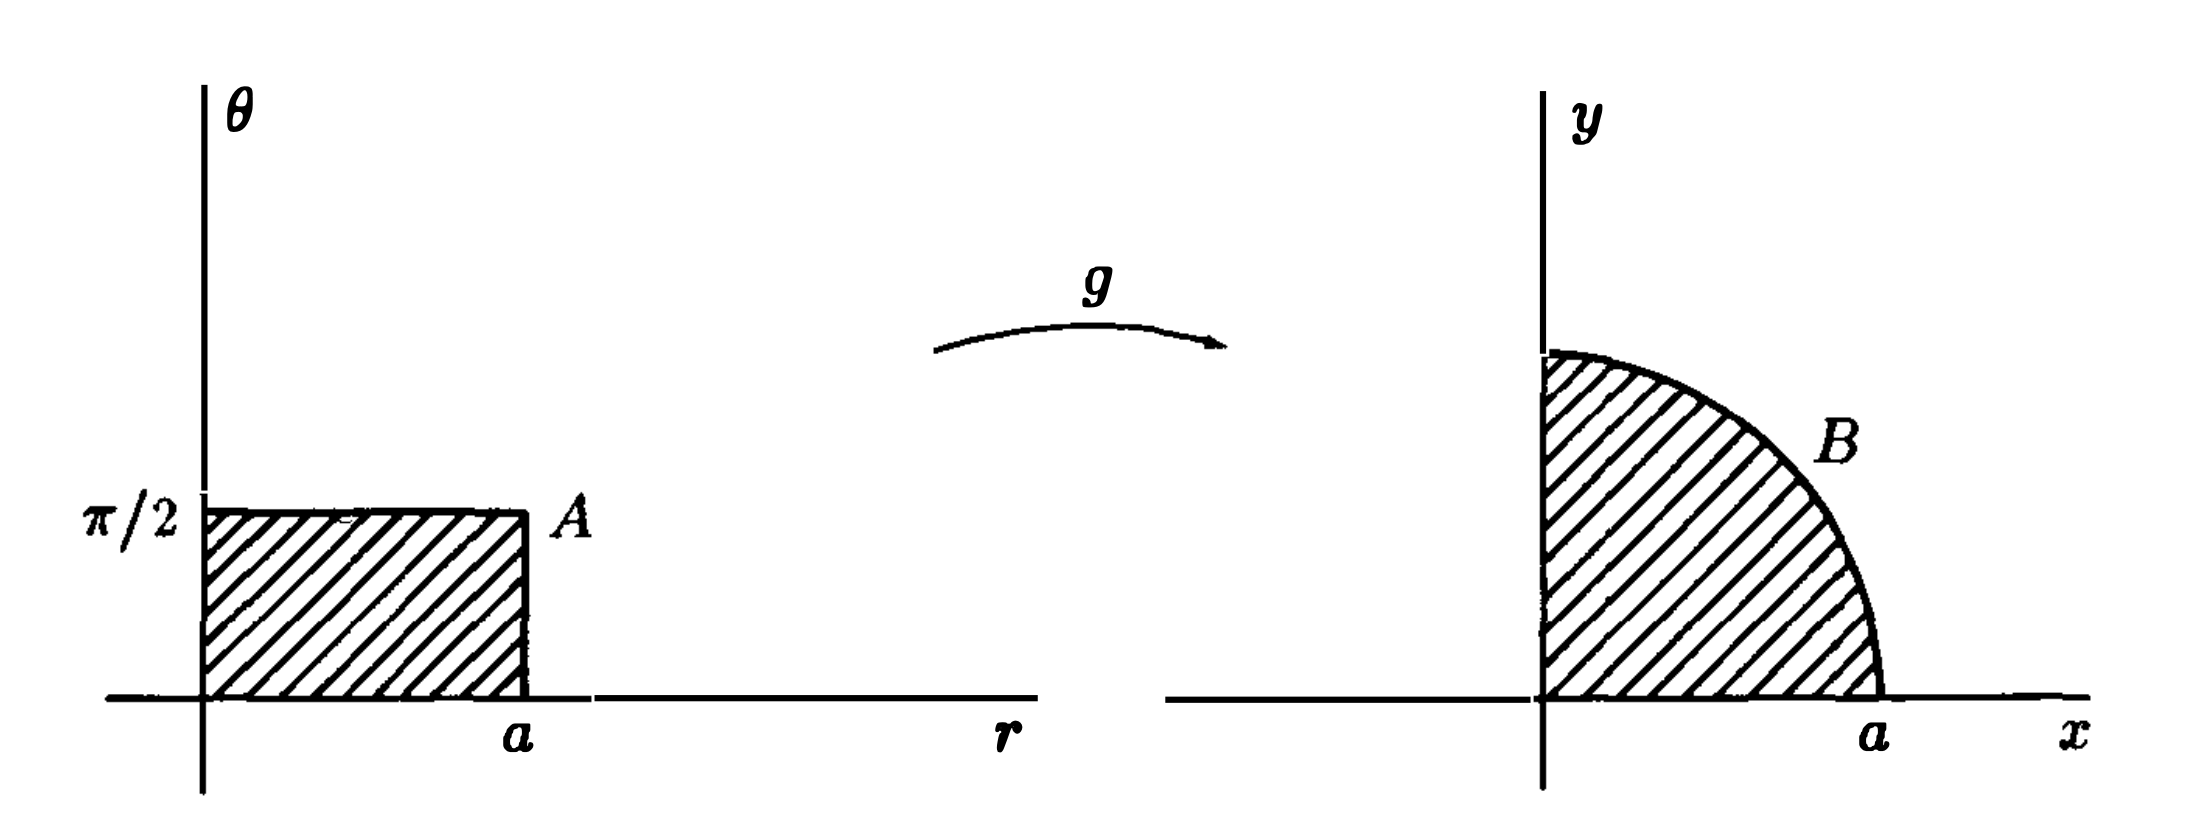
\includegraphics[scale=0.33]{images/Screenshot 2023-01-13 at 22.13.08.png}
        \caption{picture of polar coordinate transformation $g:A\to B$}
    \end{figure}
    \item If we want to integrate the function $f$ over the set
    $$W=\{(x,y):x^2+y^2<a^2\}$$
    The polar coordinate transformation cannot be a diffeomorphism now because the part where $y=0$ and $x>0$ cannot be bijective.
    However,we can define a diffeomorphism of the open $U=(0,a)\times(0,2\pi)$ with the open set $$V=\{(x,y): x^2+y^2<a^2\text{ and }x<0\text{ if }y=0\}$$
    Therefore, the integral can be evaluated as $$\int_Wf=\int_Vf=\int_Uf(r\cos\theta,r\sin\theta)\cdot r$$
    \begin{figure}[H]
        \centering
        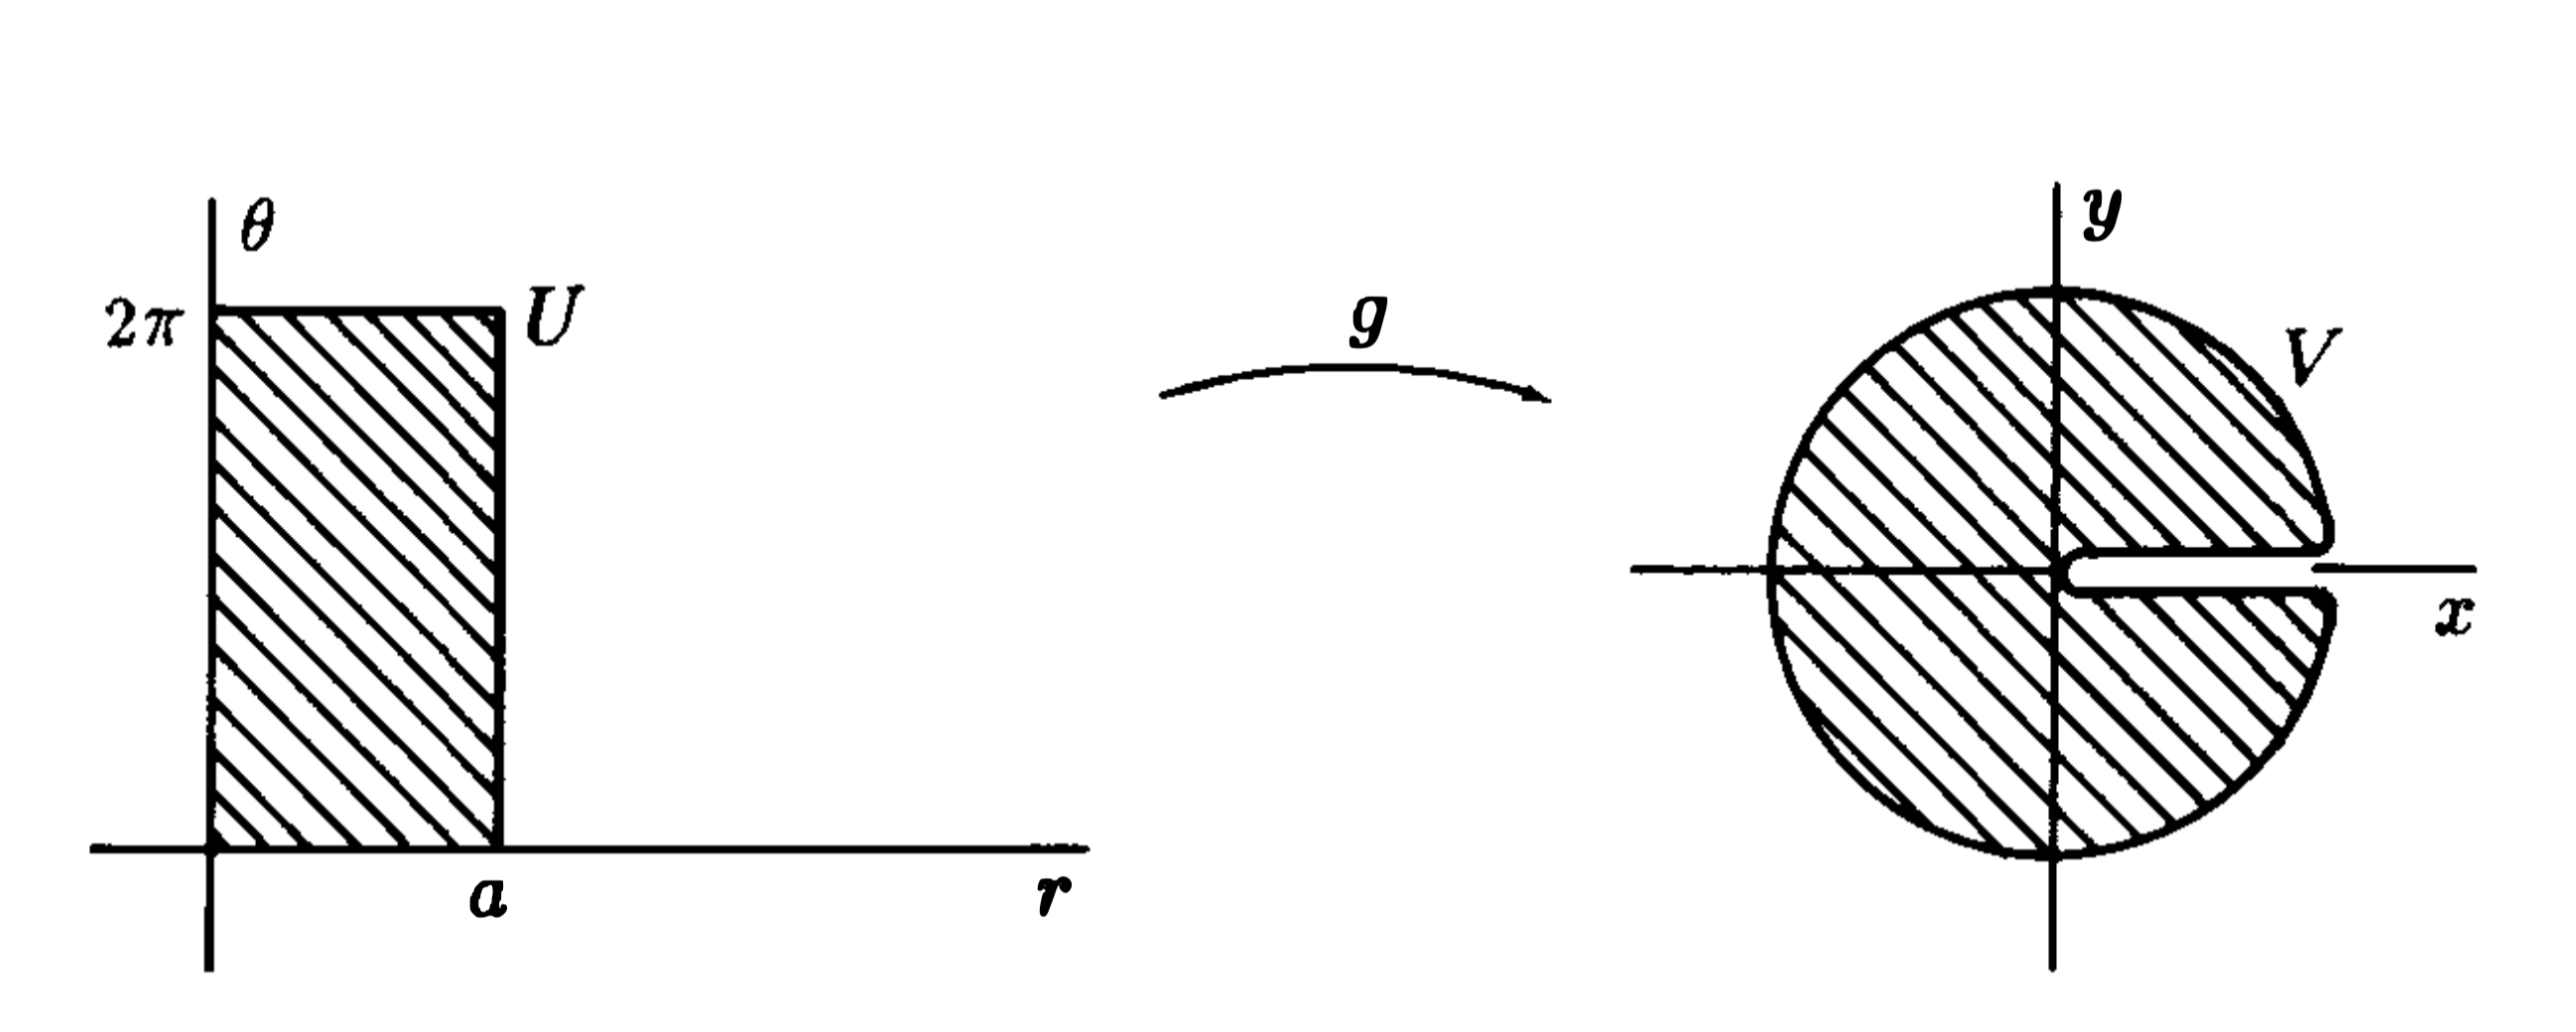
\includegraphics[scale=0.3]{images/Screenshot 2023-01-13 at 22.24.55.png}
        \caption{picture of polar coordinate transformation $g:U\to V$}
    \end{figure}
\end{itemize}


\begin{definition}
    The \underline{spherical coordinate transformation} is a function $g:\R^3\longrightarrow\R^3$ defined by 
    $$g(\rho,\phi,\theta)=(\rho\sin\phi\cos\theta,\rho\sin\phi\sin\theta,\rho\cos\phi)$$
    By computation we have
    \begin{equation*}
        \det(Dg)=\det(\begin{bmatrix}
            \sin\phi\cos\theta & \rho\cos\phi\cos\theta & -\rho\sin\phi\sin\theta\\
            \sin\phi\sin\theta & \rho\cos\phi\sin\theta & \rho\sin\phi\cos\theta\\
            \cos\phi & -\rho\sin\phi & 0
        \end{bmatrix})=\rho^2\cdot \sin\phi
    \end{equation*}
    \begin{figure}[H]
        \centering
        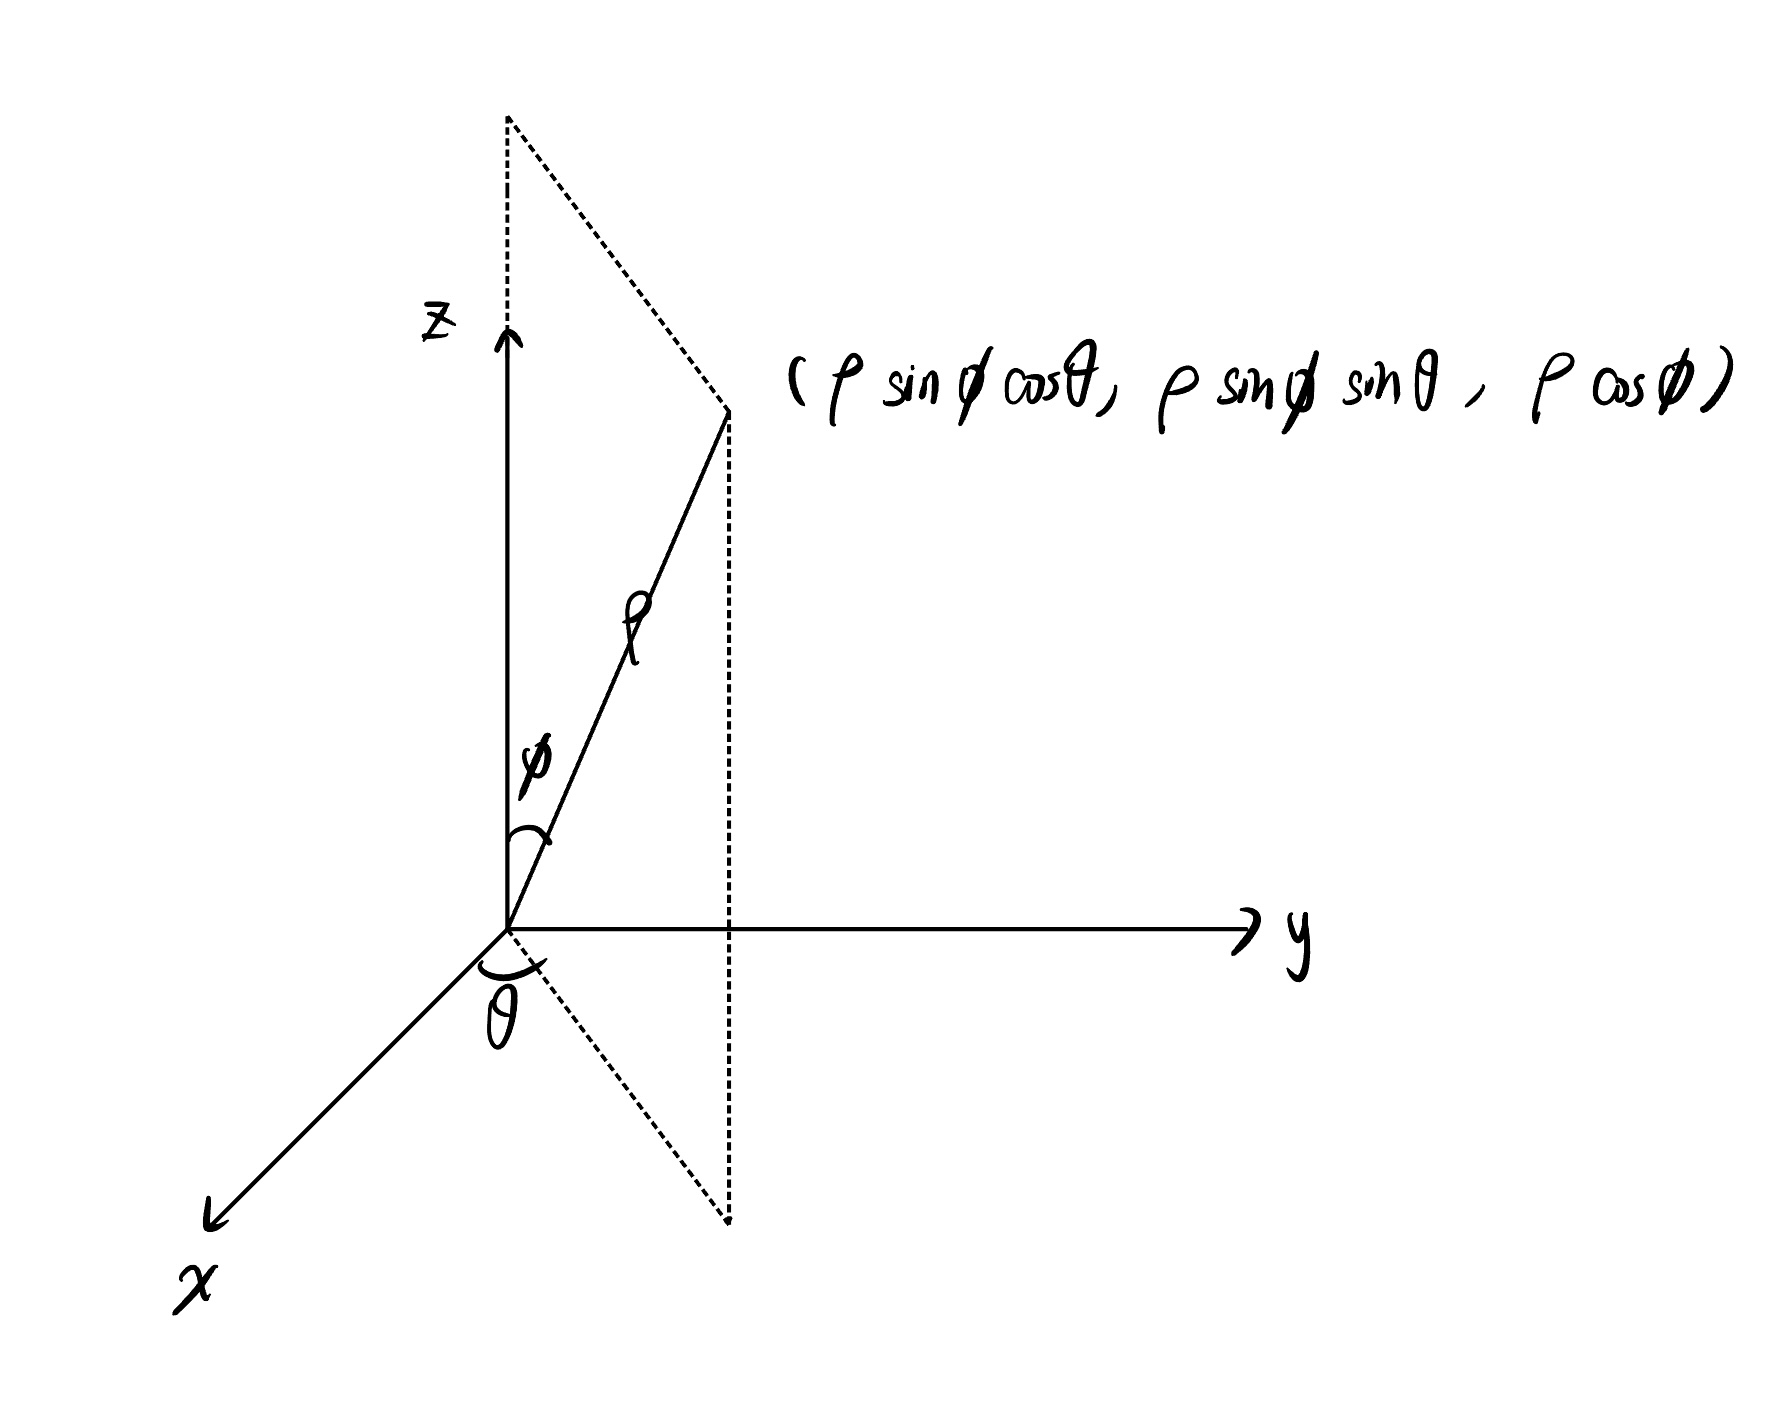
\includegraphics[scale=0.16]{images/IMG_0362.jpg}
        \caption{picture of spherical coordinate}
    \end{figure}
\end{definition}
\noindent\textbf{Example}:
\begin{itemize}
    \item Let $B$ be the open set in $\R^3$ defined by $$B=\{(x,y,z):x>0\text{ and }y>0\text{ and }x^2+y^2+z^2<a^2\}$$
    One commonly computes an integral over $B$.i.e. $\int_Bf$ by using the spherical coordinate transformation.
    Define the sets $A$ as 
    $$A=\{(\rho,\phi,\theta):0<\rho<a\text{ and }0<\phi<\pi\text{ and }0<\theta<\frac{\pi}{2}\}$$
    The map $g:A\longrightarrow B$ is a diffeomorphism. The change of variables theorem implies that $$\int_B=\int_Af(\rho\sin\phi\cos\theta,\rho\sin\phi\sin\theta,\rho\cos\phi)\cdot \rho^2\sin\phi$$
    \begin{figure}[H]
        \centering
        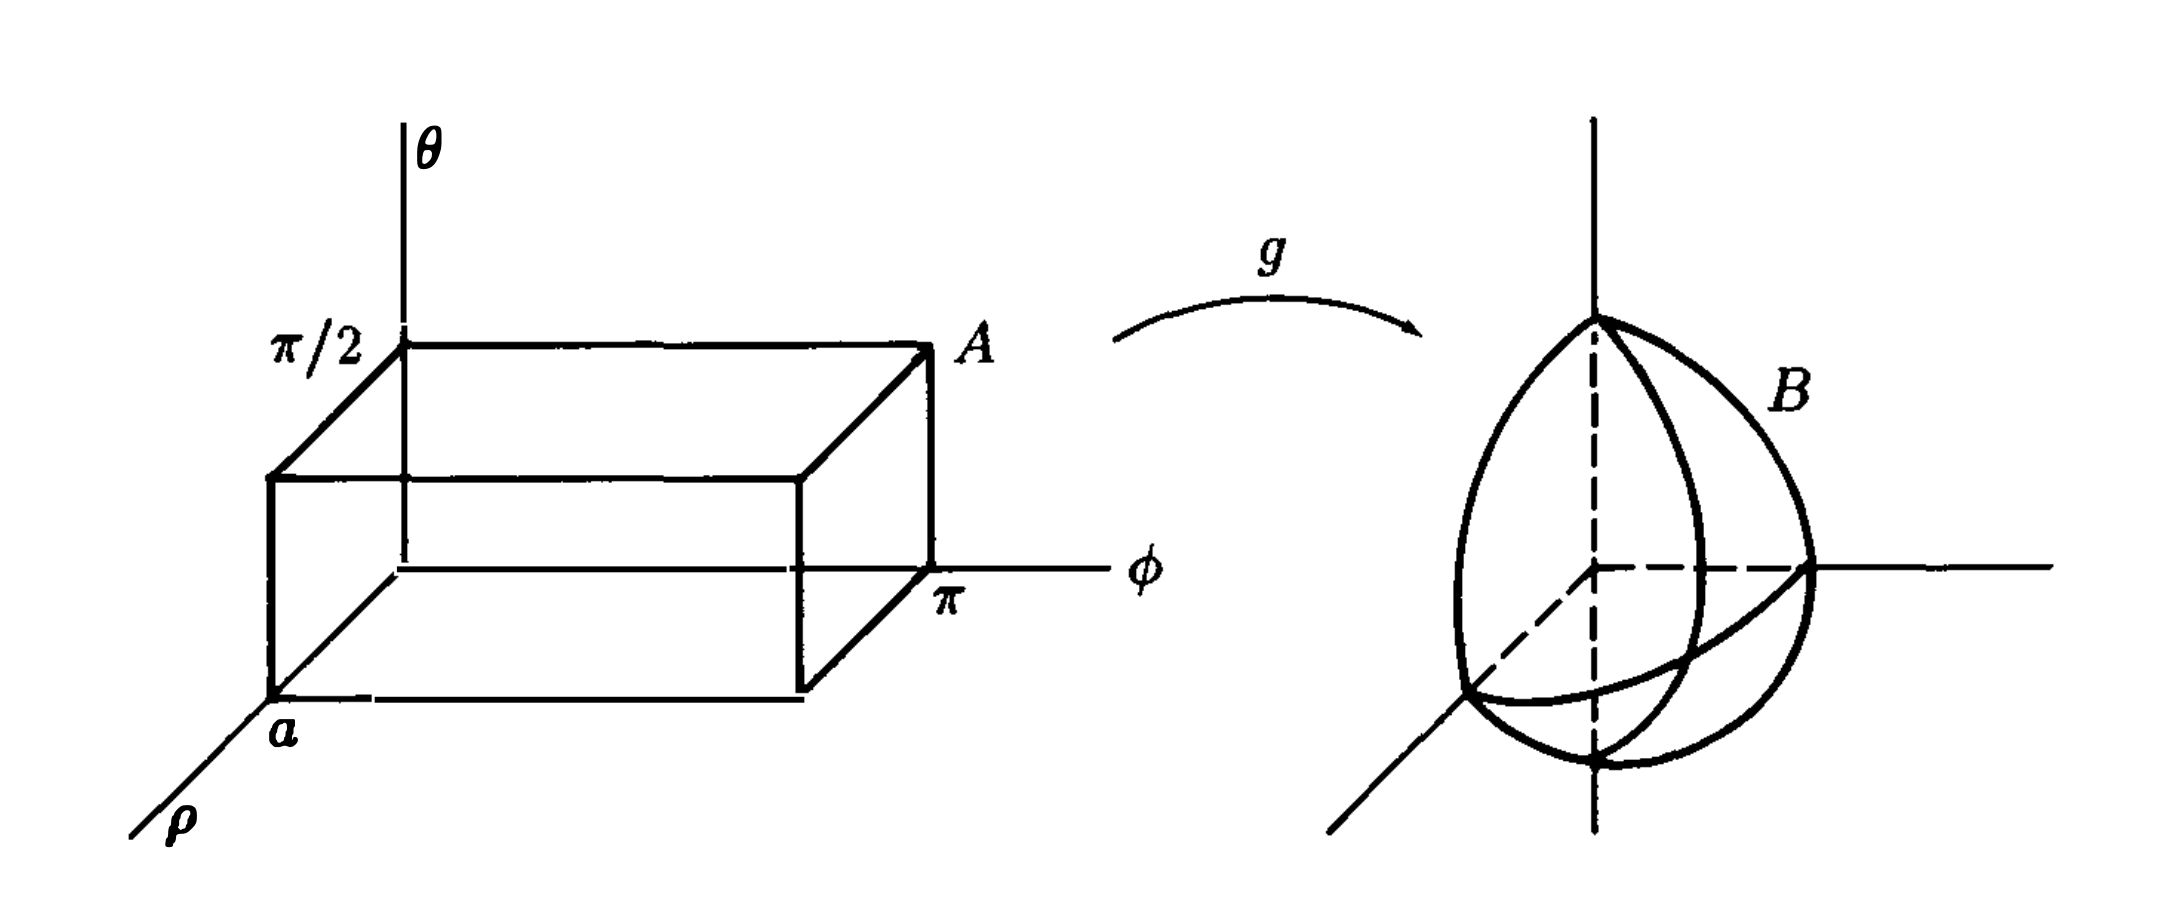
\includegraphics[scale=0.33]{images/Screenshot 2023-01-15 at 18.05.53.png}
        \caption{picture of spherical coordinate transformation $g:A\to B$}
    \end{figure}
\end{itemize}

\begin{definition}
    The \underline{Cylindrical coordinate transformation} is a function $g:\R^3\longrightarrow\R^3$ defined by
    $$g(r,\theta,z)=(r\cos\theta,r\sin\theta,z)$$
    By computation we have
    \begin{equation*}
        \det(Dg)=\det(\begin{bmatrix}
            \cos\theta & -r\sin\theta & 0\\
            \sin\theta & r\cos\theta & 0\\
            0 & 0 & 1
        \end{bmatrix})=r
    \end{equation*}
    \begin{figure}[H]
        \centering
        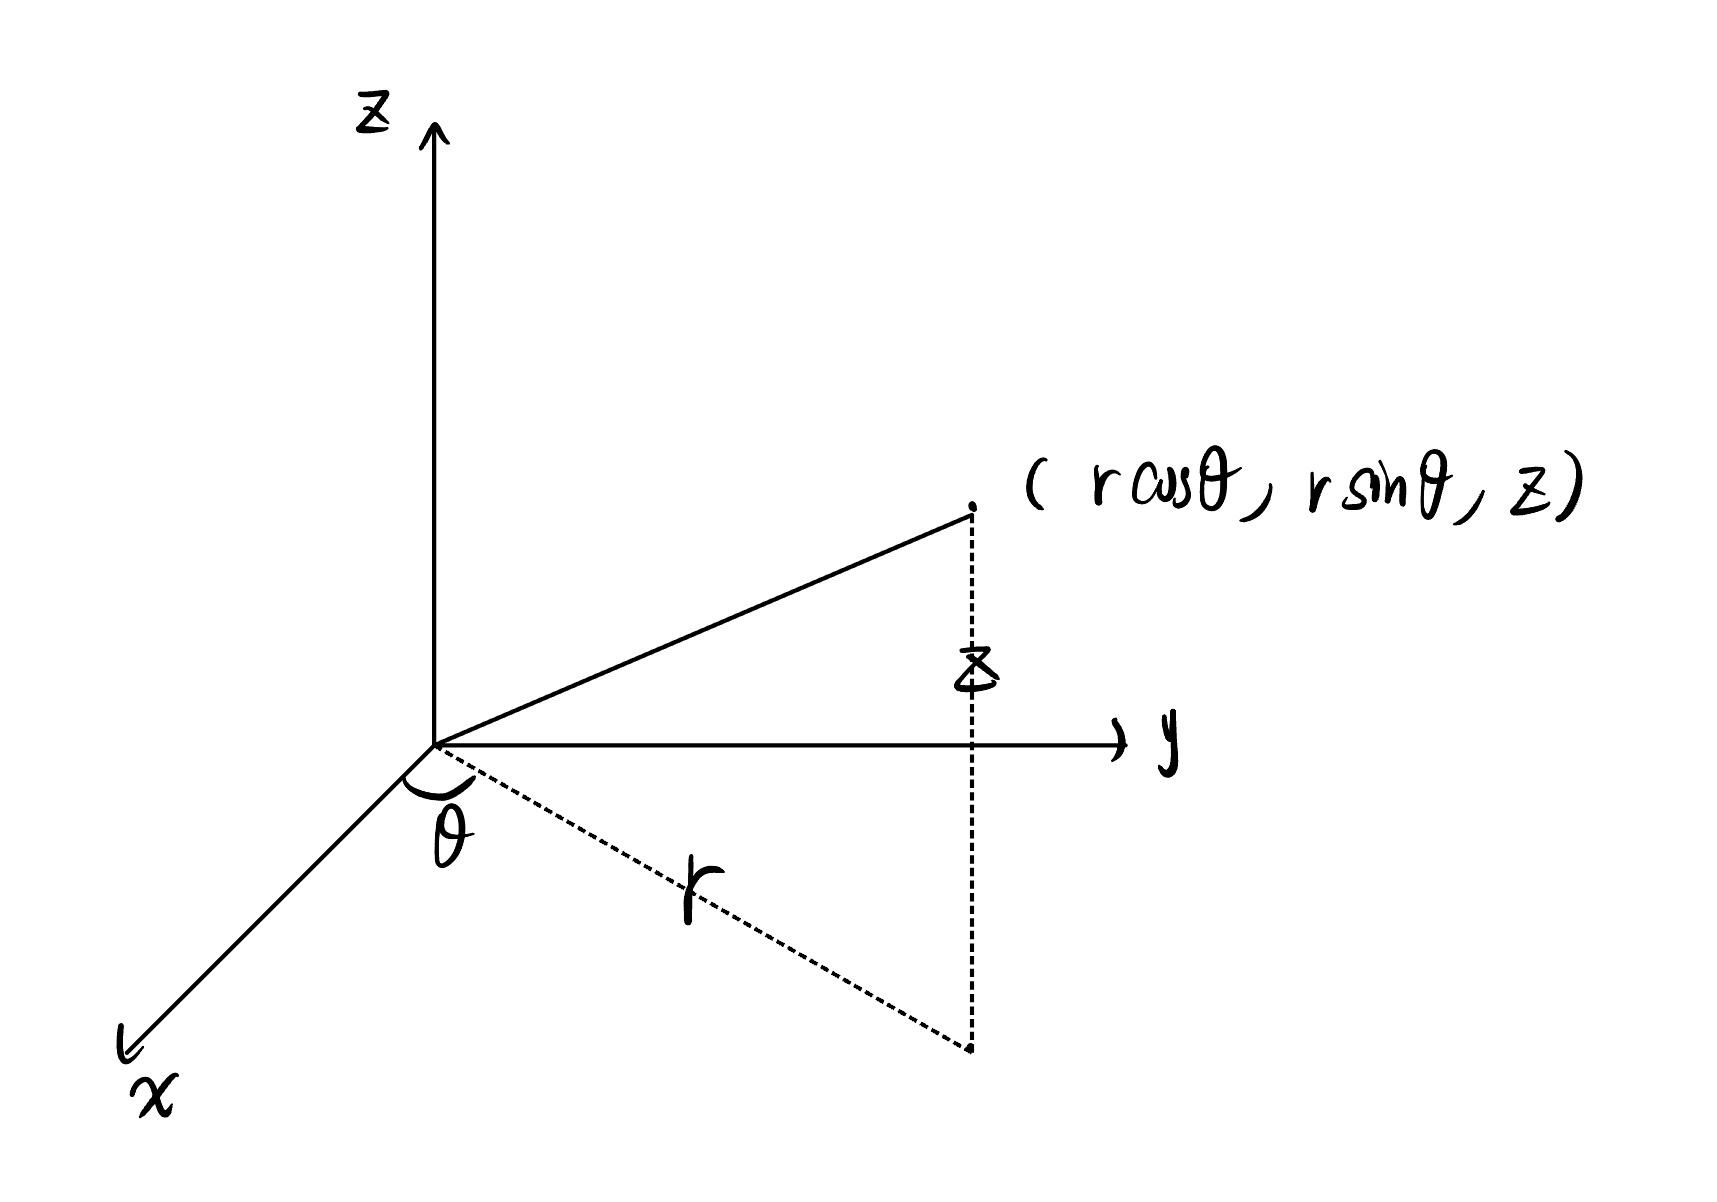
\includegraphics[scale=0.16]{images/IMG_0363.jpg}
        \caption{picture of cylindrical coordinate}
    \end{figure}
\end{definition}
\noindent\textbf{Example}:
\begin{itemize}
    \item We can use cylindrical coordinate transformation to compute the volume of a solid torus.
    Let $g$ be the cylindrical coordinate transformation. Let $$A=\{(r,\theta,z):(r-b)^2+z^2\leq a^2\text{ and }0\leq \theta\leq 2\pi\}$$
    The \underline{Solid Torus} $T$ is the image of $A$ under $g$. The volume of $T$ , say $V$, is $\int_T1$.
    \begin{figure}[H]
        \centering
        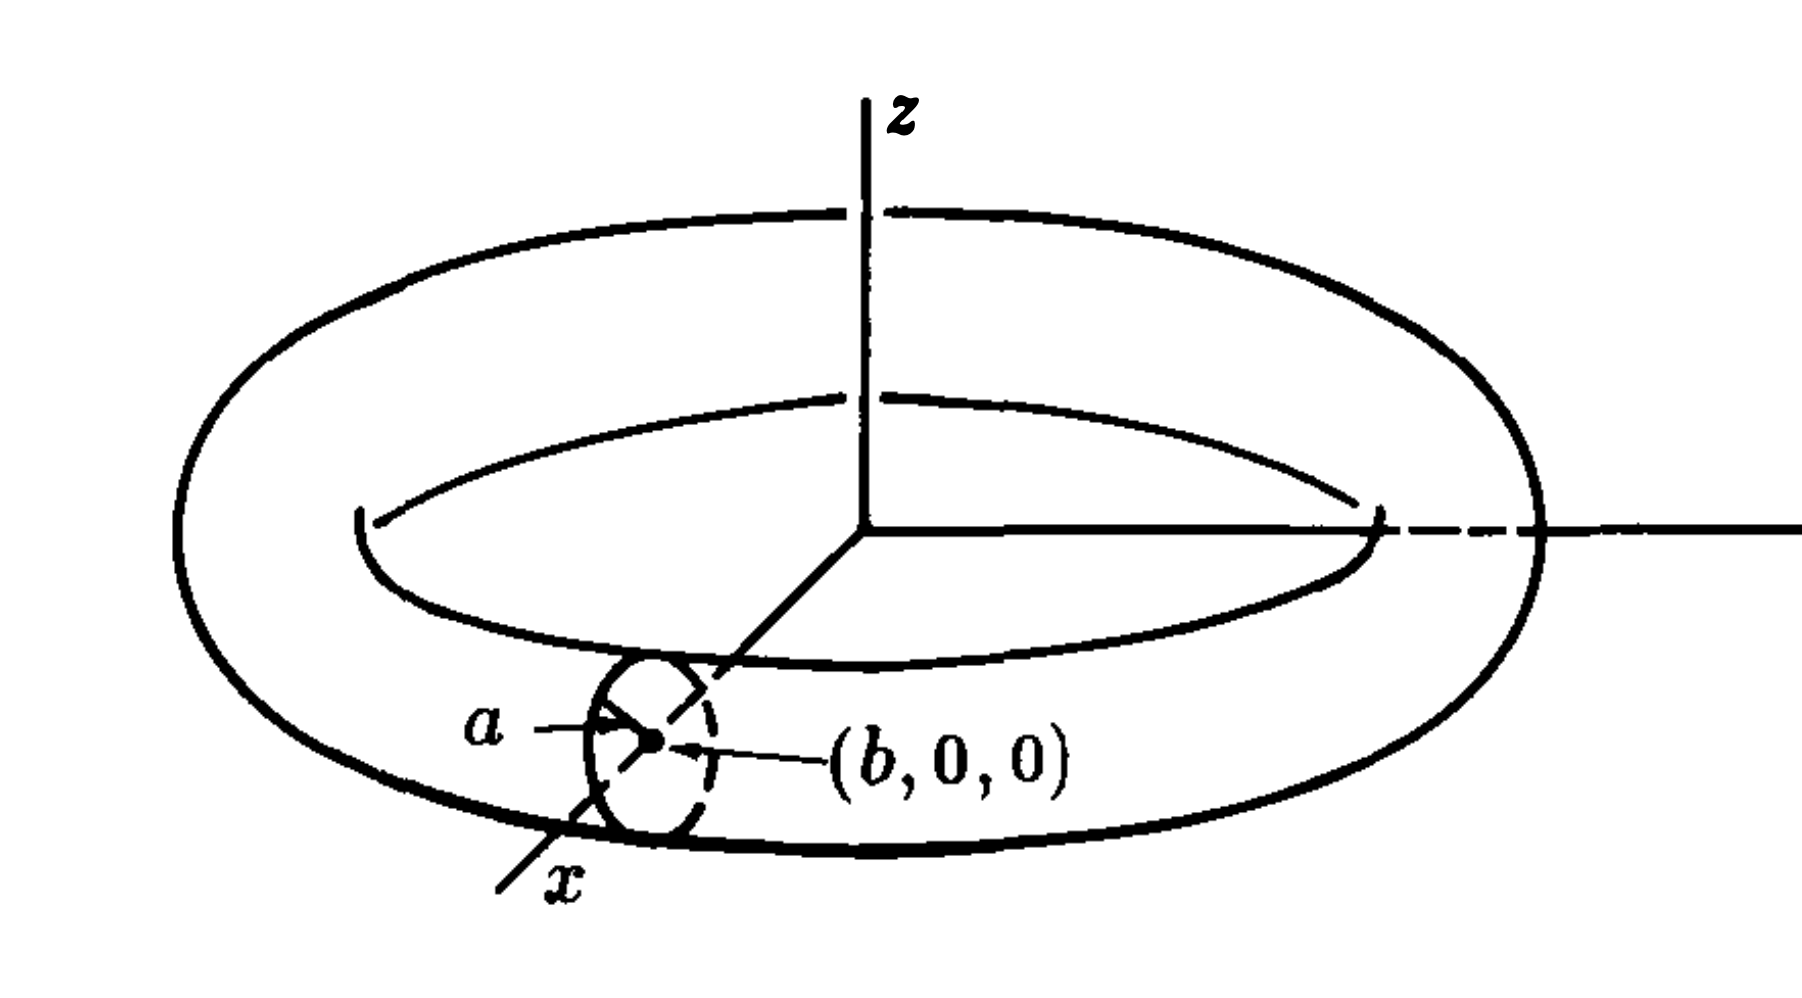
\includegraphics[scale=0.35]{images/Screenshot 2023-02-07 at 17.58.09.png}
        \caption{A solid torus in $\R^3$.}
    \end{figure}
    $$Int(A)=\{(r,\theta,z):(r-b)^2+z^2< a^2\text{ and }0< \theta< 2\pi\}$$
    Define $$T'=Int(T)\setminus\{(x,y,x)\in T: y=0 \text{ and }x>0\}$$
    Now $g:Int(A)\longrightarrow T'$ is a diffeomorphism, so we can apply the change of variable theorem.
    \begin{equation*}
        \int_{T'}1=\int_{Int(A)}(1\circ g)\cdot r
    \end{equation*}
    Since $Bd(A)$ and $Bd(T)\cup\{(x,y,x)\in T: y=0 \text{ and }x>0\}$ both have measure zero in $\R^3$ because by basic topology, their dimensions are both 2, which is less than 3.
    Therefore
    \begin{equation*}
        \begin{split}
            V &= \int_T1\\
            &=\int_{T'}1\\
            &= \int_{Int(A)}(1\circ g)\cdot r\\
            &= \int_{A}(1\circ g)\cdot r\\
            &= \int_Ah\text{\quad where }h(r,\theta,z)=r\\
            &= \int_Qh_A\text{\quad where }A\subset Q=[b-a,b+a]\times[0,2\pi]\times[-a,a]\\
            &= \int_{r=b-a}^{r=b+a}\int_{\theta=0}^{\theta=2\pi}\int_{z=-a}^{z=a}h_A\di z \di \theta \di r\\
            &=\int_{r=b-a}^{r=b+a}\int_{\theta=0}^{\theta=2\pi}2\sqrt{a^2-(r-b)^2}\cdot r \di \theta\di r\\
            &=\int_{r=b-a}^{r=b+a}4\pi\cdot r \cdot \sqrt{a^2-(r-b)^2}\di r\\
            &=2\pi^2a^2b
        \end{split}
    \end{equation*}
\end{itemize}

\subsection{n-dimensional Cone, Ball in $\R^n$}

\begin{definition}
    Given a rectifiable set $S$ in $\R^n$. We define the \underline{centroid} of $S$ to be the point $c(S)\in \R^n$ such that
    for each $k\in\{1,\cdots,n\}$ $$c_k(S)=\frac{1}{v(S)}\int_S\pi_k$$ where $\pi_k$ is the projection function.
\end{definition}

\begin{definition}
    We say $S$ is \underline{symmetric} with respect to the subspace $x_k=0$ of $\R^n$ if the transformation $$h(x)=(x_1,\cdots,x_{k-1},-x_k,x_{k+1},\cdots,x_n)$$ carries $S$ onto itself.
\end{definition}

\begin{theorem}
    If $S$ is symmetric with respect to the subspace $x_k=0$ of $\R^n$, then $c_k(S)=0$.
\end{theorem}

\begin{definition}
    Let $A$ be an open rectifiable set in $\R^{n-1}$. Given the point $p\in\R^n$ with $p_n>0$. 
    Define $$S=\{x\in\R^n:x=(1-t)a+tp\text{ where }a\in A\times0\text{ and }0<t<1\}$$
    Then $S$ is the union of all open line segments in $\R^n$ joining $p$ to points of $A|times0$. The closure of $S$ is called the \underline{cone} with base $\overline{A}\times0$ and vertex $p$.
    \begin{figure}[H]
        \centering
        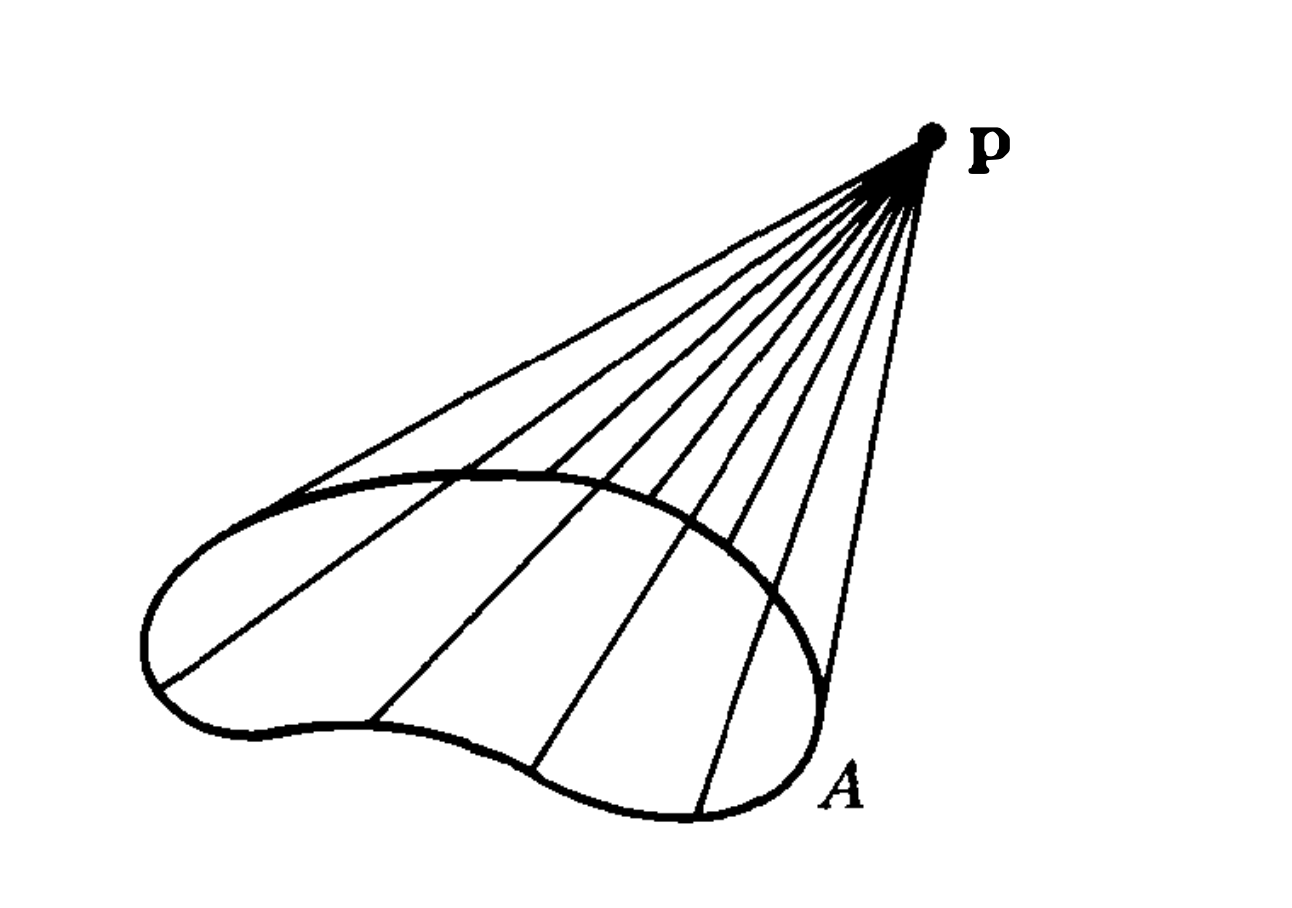
\includegraphics[scale=0.3]{images/Screenshot 2023-01-21 at 16.55.12.png}
        \caption{A cone in $\R^3$}
    \end{figure}
\end{definition}
\noindent\textbf{Remark}:
\begin{itemize}
    \item Just like the coordinate transformations we have learnt, we can use $n$ parameters $(m_1,\cdots,m_n)$ to represent any points $x=(x_1,\cdots,x_n)$ in the open cone $S$.
    Given $x\in S$, we can project $x$ along the line joining $p,x$ to a point $(m_1,\cdots,m_{n-1})$ on the hyperplane $A$, let $m_n$ denote the relative hight on the line. Therefore 
    $$g(m_1,\cdots,m_{n-1},m_n)=(m_n(p_1-m_1)+m_1,\cdots,m_n(p_{n-1}-m_{n-1})+m_{n-1},p_nm_n)$$
    \item $g$ is indeed a diffeomorphism because 
    $$\det(Dg(\vec{m}))=\det(\begin{bmatrix}
        -m_n+1& 0 & \cdots & 0 & p_1-m_1\\
        0 & -m_n+1 & \cdots & 0 & p_2-m_2\\
        \vdots & \vdots & \ddots & \vdots & \vdots\\
        0 & 0 & \cdots & -m_n+1 & p_{n-1}-m_{n-1}\\
        0 & 0 & \cdots & 0 & p_n
    \end{bmatrix})=(-m_n+1)^{n-1}>0$$
    \item If we want to integrate a fuction $f:S\longrightarrow\R$, we can use the change of variable theorem to convert the integral to function $(f\circ g)(-m_n+1)^{n-1}$ on the set $A\times(0,1)$.
\end{itemize}

\begin{theorem}
    Given the volume $v(A)$, we can get $$v(S)=\frac{p_n}{n}v(A)$$
\end{theorem}
\noindent\textbf{Remark}:
\begin{itemize}
    \item This formula corresponds the formula we learnt for 3-dimensional cone in elementary school.
\end{itemize}

\begin{theorem}
    The centroid $c(S)$ of $S$ lies on the line segment joining $c(A)$ and $p$. Explicitly $$c(S)=\frac{n}{n+1}(c(A),0)+\frac{1}{n+1}p$$
\end{theorem}

\begin{definition}
    We will denote the closed ball of radius $a$ in $\R^n$ by $B^n(a)$.
    We will use the general term $\lambda_n$ to denote $v(B^n(1))$.
\end{definition}

\begin{theorem}
    $$v(B^n(a))=v(B^n(1))\cdot a^n=\lambda_na^n$$
\end{theorem}

\begin{theorem}
    $\lambda_n$ has the recurrsion $$\lambda_n=\frac{2\pi}{n}\lambda_{n-2}$$
\end{theorem}

\begin{theorem}
    \begin{equation}
        \lambda_n=
        \begin{cases}
            \frac{(2\pi)^{\frac{n}{2}}}{n!!}\text{\quad for n even}\\
            \frac{2(2\pi)^{\frac{n-1}{2}}}{n!!}\text{\quad for n odd}
        \end{cases}
    \end{equation}
\end{theorem}

\begin{definition}
    We use $B_+^n(a)$ to denote the upper half n-ball.
\end{definition}

\begin{theorem}
    \begin{equation}
        \begin{split}
            c(B_+^n(a)) &= (0,\cdots,0,\frac{2a}{n+1}\times\frac{\lambda_{n-1}}{\lambda_n})\\
            &=\frac{n}{n+1}(0,0,c(B_+^{n-2}(a)))
        \end{split}
    \end{equation}
\end{theorem}

\subsection{The Meaning of Determinant}

\begin{definition}
    Let $A$ be an n by n matrix. Let $h:\R^n\longrightarrow\R^n$ be the linear transformation $h(x)=A\cdot x$. Then
    $$v(h(S))=|\det(A)|\cdot v(S)$$
\end{definition}

\begin{definition}
    Let $\vec{a_1},\cdots,\vec{a_k}$ be independent vectors in $\R^n$. We define the \underline{k-dimensional parallelopiped} to be 
    $$\mathcal{P}(\vec{a_1},\cdots,\vec{a_k})=\{x=c_1\vec{a_1}+\cdots+c_k\vec{a_k}: 0\leq c_i \leq 1\}$$
    The vectors $\vec{a_1},\cdots,\vec{a_k}$ are called the \underline{edges} of $\mathcal{P}$.
    \begin{figure}[H]
        \centering
        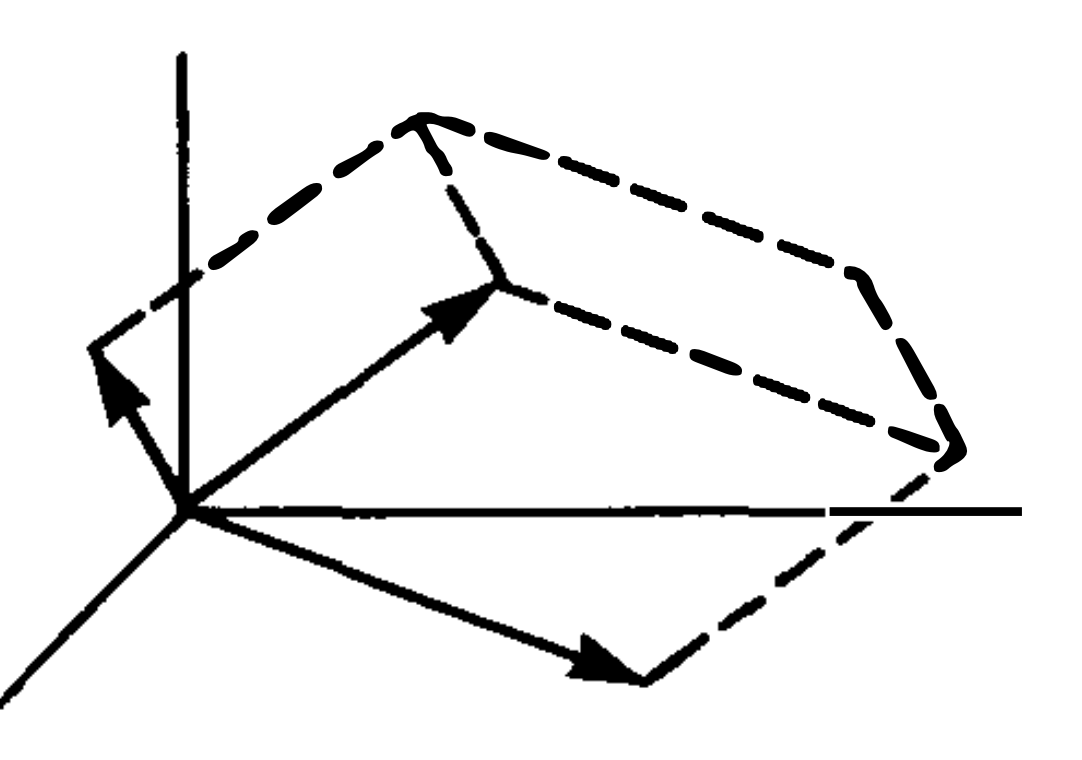
\includegraphics[scale=0.3]{images/Screenshot 2023-01-15 at 23.58.43.png}
        \caption{picture of a parallelopiped in $\R^3$}
    \end{figure}
\end{definition}

\begin{theorem}[The volume of n-dim parallelopiped in $\R^n$]
    Let $\vec{a_1},\cdots,\vec{a_n}$ be independent vectors in $\R^n$.
    Let $A=[\vec{a_1}\cdots\vec{a_n}]$ be the n by n matrix with columns $\vec{a_1},\cdots,\vec{a_n}$. Then
    $$v(\mathcal{P}(\vec{a_1},\cdots,\vec{a_n}))=|\det(A)|$$
\end{theorem}
\begin{corollary}
    Let $\vec{a_1},\vec{a_2},\vec{a_3}$ be edges of a parallelopiped $\mathcal{P}(\vec{a_1},\vec{a_2},\vec{a_3})$ in $\R^3$. Then
    $$\mathcal{P}(\vec{a_1},\vec{a_2},\vec{a_3})=|\det(\begin{bmatrix}
        \vec{a_1}&\vec{a_2}&\vec{a_3}
    \end{bmatrix})|=|\vec{a_1}\cdot(\vec{a_2}\times\vec{a_3})|$$
\end{corollary}
\noindent\textbf{Remark}:
\begin{itemize}
    \item Intuitively, $\vec{a_2}\times\vec{a_3}$ is the area of the base side, $\vec{a_1}$ is the height.
\end{itemize}

\begin{definition}
    Let $V$ be an n-dimensional vector space. An n-tuple $(\vec{a_1},\cdots,\vec{a_n})$ of independent vecors in $V$ is called an \underline{n-frame} in $V$.
\end{definition}

\begin{definition}
    In $\R^n$, we call a frame $(\vec{a_1},\cdots,\vec{a_n})$
    \begin{itemize}
        \item \underline{right-handed} if $\det(\begin{bmatrix}
            \vec{a_1} & \cdots & \vec{a_n}
        \end{bmatrix})>0$
        \item \underline{left-handed} if $\det(\begin{bmatrix}
            \vec{a_1} & \cdots & \vec{a_n}
        \end{bmatrix})<0$
    \end{itemize}
    \begin{figure}[H]
        \centering
        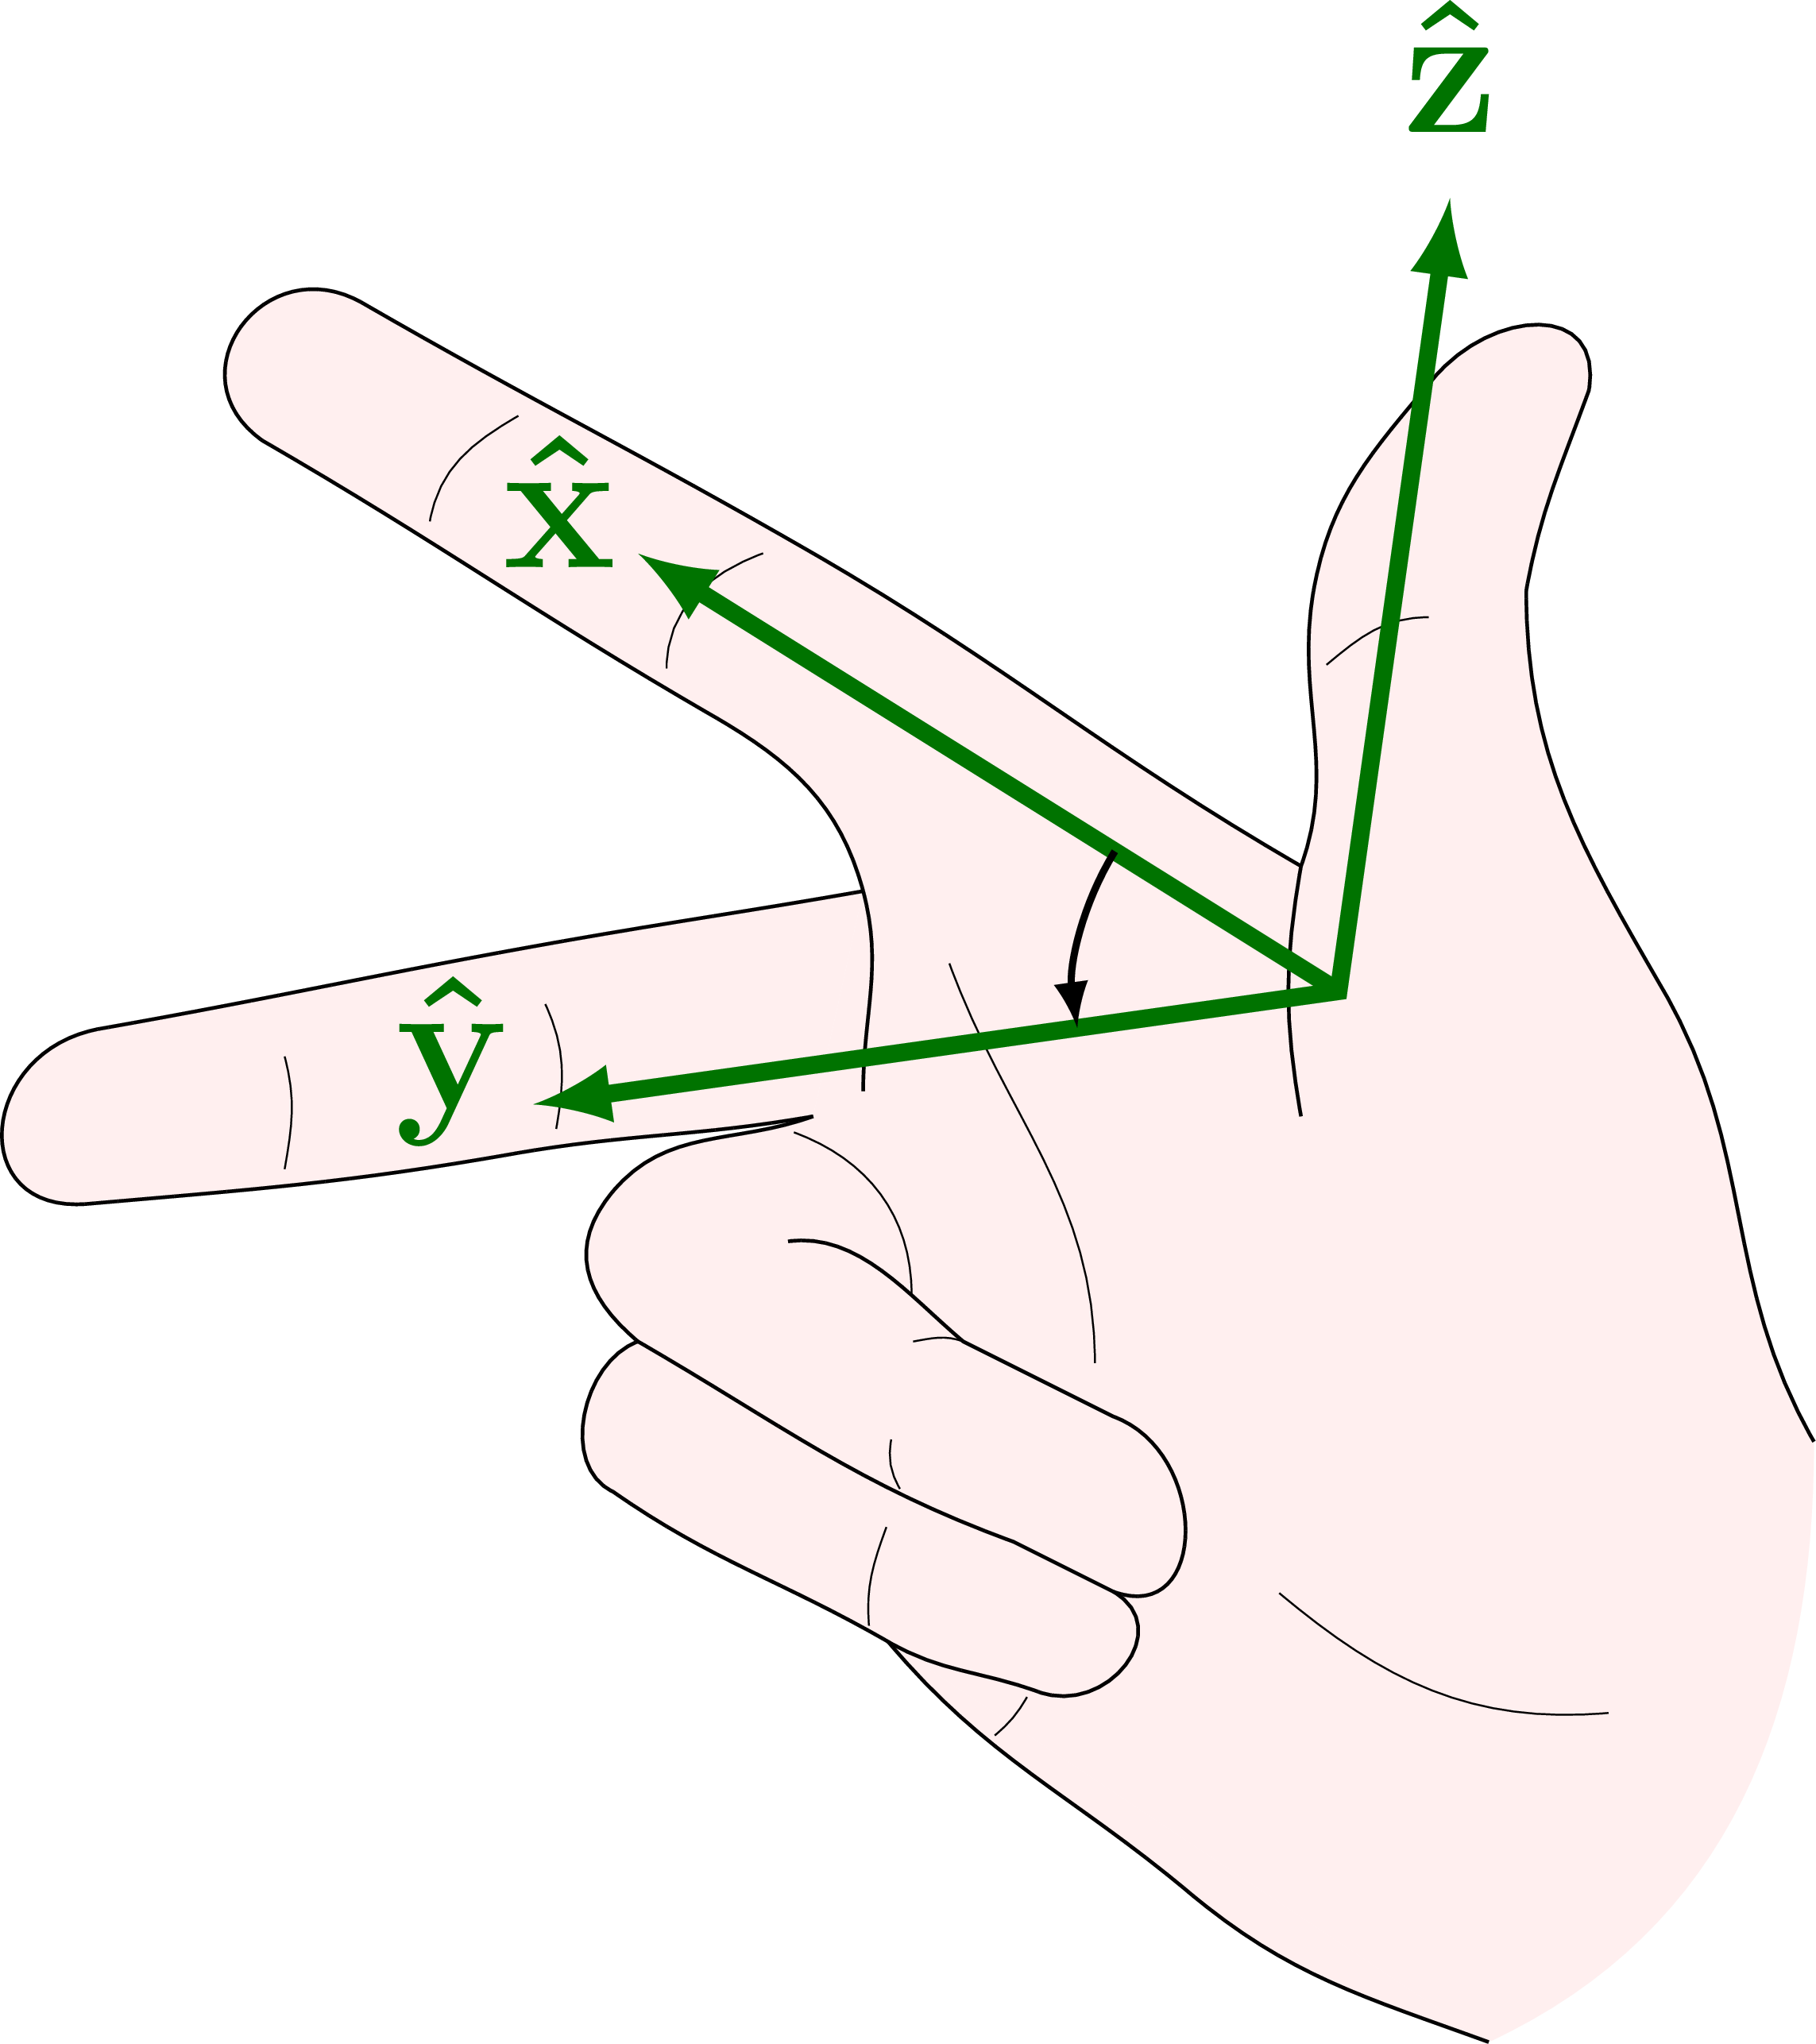
\includegraphics[scale=0.08]{images/righthand_rule-002.png}
        \caption{picture of a right-handed frame}
    \end{figure}
\end{definition}

\begin{definition}
    In $\R^n$ we have two \underline{orientations}:
    \begin{itemize}
        \item the collection of all right-handed frames in $\R^n$
        \item the collection of all left-handed frames in $\R^n$
    \end{itemize}
    Given a isomorphism $T:\R^n\longrightarrow V$ we can define the two \underline{orientations} of $V$:
    \begin{itemize}
        \item the collection of the forms $(T(\vec{a_1},\cdots,\vec{a_n}))$ where $(\vec{a_1},\cdots,\vec{a_n})$ is a right-handed frame in $\R^n$.
        \item the collection of the forms $(T(\vec{a_1},\cdots,\vec{a_n}))$ where $(\vec{a_1},\cdots,\vec{a_n})$ is a left-handed frame in $\R^n$.
    \end{itemize}
\end{definition}

\begin{theorem}
    Let $C$ be a non-singular n by n matrix. Let $h:\R^n\longrightarrow\R^n$ be the linear transformation $h(x)=C\cdot x$. Let $(\vec{a_1},\cdots,\vec{a_n})$ be a frame of $\R^n$.
    \begin{itemize}
        \item If $\det(C)>0$, then the frame $(\vec{a_1},\cdots,\vec{a_n})$ and the frame $(h(\vec{a_1}),\cdots,h(\vec{a_n}))$ belong to the same orientation. In this case, we say $h$ is \underline{orientation-preserving}.
        \item If $\det(C)<0$, then the frame $(\vec{a_1},\cdots,\vec{a_n})$ and the frame $(h(\vec{a_1}),\cdots,h(\vec{a_n}))$ belong to the opposite orientation. In this case, we say $h$ is \underline{orientation-reversing}.
    \end{itemize}
\end{theorem}

\subsection{Isometries Preserve Volume}

\begin{definition}\
    \begin{enumerate}
        \item The set $\{\vec{a_1},\cdots,\vec{a_k}\}$ is \underline{orthogonal} if $\forall i,j\in\{1,\cdots,k\}.i\neq j\implies \innerp{\vec{a_i}}{\vec{a_j}}=0$
        \item The set $\{\vec{a_1},\cdots,\vec{a_k}\}$ is \underline{orthonormal} if it is orthogonal and $\forall i\in\{1,\cdots,k\}.\innerp{\vec{a_i}}{\vec{a_i}}=1$
    \end{enumerate}
\end{definition}

\begin{definition}
    An n by n matrix $A$ is called an \underline{orthogonal matrix} if the columns of $A$ form an orthonormal set. A linear transformation $h(x)=A\cdot x$ is called an \underline{orthogonal transformation} if $A$ is an orthogonal matrix.
\end{definition}

\begin{theorem}
    A matrix $A$ is orthogonal if and only if $A^T=A^{-1}$.
\end{theorem}

\begin{corollary}
    If $A$ is orthogonal, then $\det(A)=1\text{ or }-1$.
\end{corollary}

\begin{theorem*}
    All the orthogonal n by n real matrix forms a group, which is called \underline{orthogonal group}, denoted as $O(n,\R)$.
\end{theorem*}

\begin{definition}
    The function $h:\R^n\longrightarrow\R^n$ is called a \underline{(euclidean) isometry} if for all $x,y\in\R^n$
    $$\norm{h(x)-h(y)}=\norm{x-y}$$
\end{definition}

\begin{theorem}
    Let $h:\R^n\longrightarrow\R^n$ that fix the origin.($h(0)=0$)
    \begin{enumerate}
        \item $h$ is an isometry if and only if $h$ preserves dot product.
        \item $h$ is an isometry if and only if $h$ is an orthogonal transformation.
    \end{enumerate}
\end{theorem}

\begin{theorem}
    $h$ is an isometry if and only if it equals an orthogonal transformation followed by a translation, that is, if and only if $h$ has the form $$h(x)=A\cdot x+p$$
    where $A$ is an orthogonal matrix.
\end{theorem}

\begin{theorem}
    If $h$ is an isometry and $S$ is a rectifiable set, then $h(S)$ is rectifiable and $v(h(S))=v(S)$.
\end{theorem}